\documentclass{article}
\usepackage[utf8]{inputenc}
\usepackage{graphicx}
\usepackage{fancyhdr}
\usepackage{geometry}
\usepackage{amsmath}
\usepackage{amssymb}


\geometry{left = 2.5cm, right=2.5cm, bottom=2.5cm, top=2.5cm}

\title{3806ICT - Week 3 Lab}
\author{Nick van der Merwe - s5151332 - nick.vandermerwe@griffithuni.edu.au}

\pagestyle{fancy}
\renewcommand{\headrulewidth}{1pt}
\fancyhf{}
\rhead{3806ICT - Lab 3}
\chead{Griffith University}
\lhead{Nick van der Merwe - s5151332}
\rfoot{Page \thepage}
\newcommand\tab[1][1cm]{\hspace*{#1}}

\begin{document}
\maketitle

%==============================================================================
\section*{Question 1}
\textbf{\textit{
    \tab Give  definitions  of  locomotion  and  manipulation.  What  are  their shared features and differences?  
}} \\ \\
Locomotion is defined as a robot's ability to move itself by exerting force on 
the environment whereas manipulation is its ability to move objects by 
exerting force upon them.
%==============================================================================
\section*{Question 2}
\textbf{\textit{
    \tab What are advantages and disadvantages of legged robots?
}} \\ \\
Easiest format to see this in would be lists:
\subsubsection*{Advantages}
\begin{itemize}
    \item They can go over more complicated obstacles without 
        getting stuck (slanted ground, steps, et cetera)
    \item Causes less damage to terrain than wheeled robots
\end{itemize}
\subsubsection*{Disadvantages}
\begin{itemize}
    \item Movement speed
    \item Complexity - actuators and structure are a lot more complicated
    \item Harder to control - must consider balance and stability
    \item Less energy efficient due to:
    \begin{itemize}
        \item Terrain
        \item Centre of gravity moves while walking
        \item Picking up the legs
    \end{itemize}
\end{itemize}
%==============================================================================
\section*{Question 3}
\textbf{\textit{
    \tab What is DOF? If a robot can only move forward and backward, 
    how many DOFs does it have? In most cases, how many DOFs does a robot leg has?
}} \\ \\
DOF stands for \textbf{d}egrees \textbf{o}f \textbf{f}reedom, and its defined by the
number of joins in each leg. To have a leg that only moves forwards and backwards,
it would have two joints: this is because its limited to doing a lift and swing motion.
To move backwards it just swings in the other direction than normal. Most robot legs
have three joints.
%==============================================================================
\newpage
\section*{Question 4}
\textbf{\textit{
    \tab What is a gait of a legged robot? Enumerate all lift and release 
    events of a robot with 4 legs. Give two examples of gaits for such a robot.
}} \\ \\
Our formula to find how many states there are is $2^k = 2^4 = 16$ states.
\begin{figure}[ht]
    \centering
    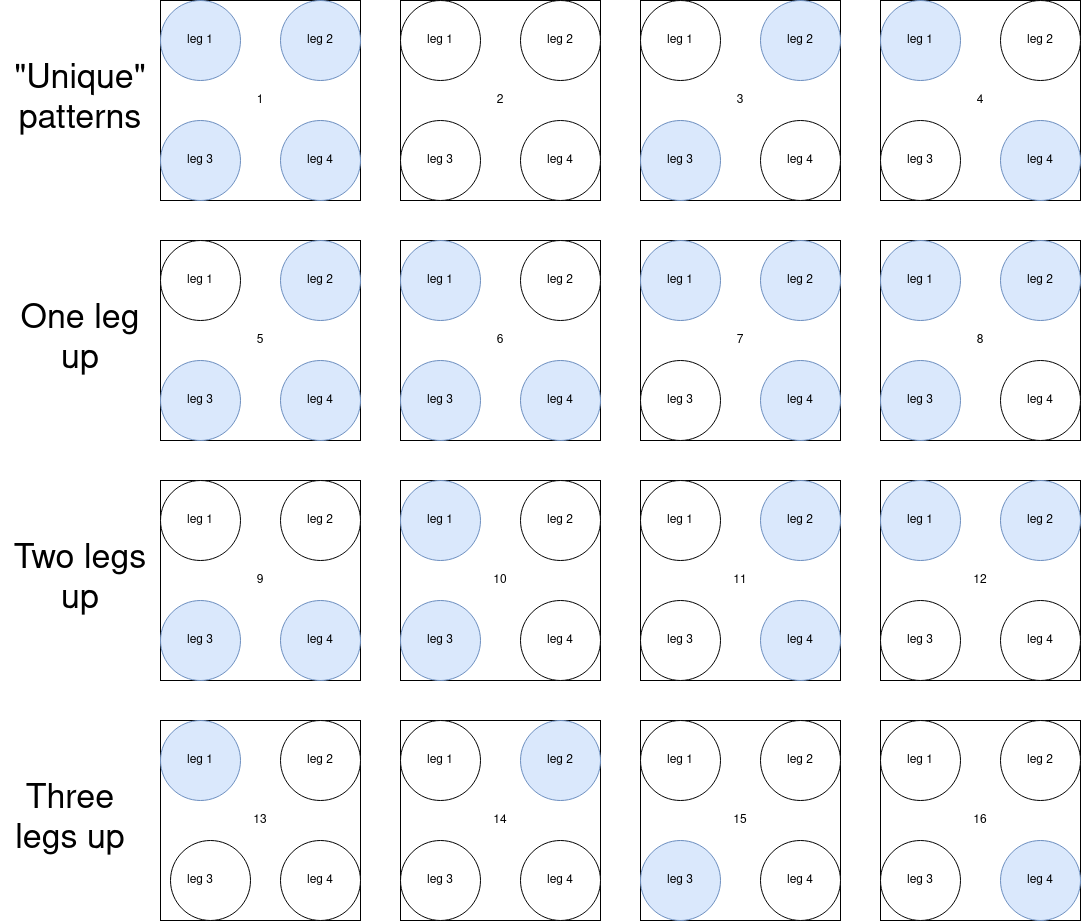
\includegraphics[width=0.5\textwidth]{img/gait.png}
    \caption{Blue means a leg is down and white is the leg is up}
\end{figure}

Now to depict gaits, we can consider the way that a horse moves since it has a walk,
trot, canter and gallop. Let's do the walk and gallop.
\begin{figure}[ht]
    \centering
    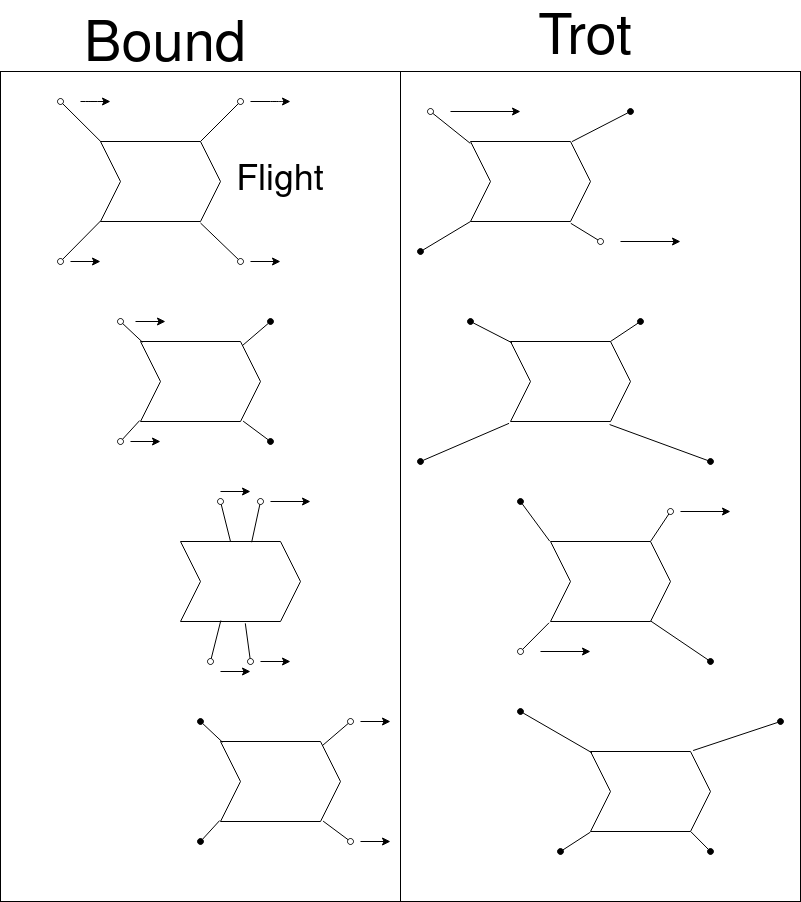
\includegraphics[width=0.65\textwidth]{img/gait-walk}
    \caption{The sources used are from http://allaboutanimation.com/ and 
    http://theanimatorssurvivalkit.com/}
\end{figure}
%==============================================================================
\section*{Question 5}
\textbf{\textit{
    \tab Formulate the Monkey and Banana Problem in STRIPS:A monkey is at location A in a lab. There is a box in location C. The monkey wants the bananas that are hanging from the ceiling in location B, but it needs to move the box and climb onto it in order to reach them
}} \\ \\
%//////////////////////////
There's a couple of things to clarify here before we start. First of all, like
the example in the slides the hand is not an object in the domain, meaning the 
monkey shouldn't be either. \\
\tab Secondly, the goal state is slightly ambigious.
By the wording of the problem it could mean that the monkey only wants to be able
to reach them, but for this lets define the operation of grabbing bananas as well
(therefore the goal is just having the bananas).
This also brings another issue to light, should the goal state include the location
and that the monkey is standing on the box? Lets define this as the monkey has bananas, the box is at B and is holding the bananas. \\
\tab Another question is whether the bananas are counted as an object.
Technically the monkey doesn't actually interact with them (i.e. picking them up) as it simply gains the state of having the bananas. 
For our case lets say the bananas are an object and the goal is carrying(bananas) 
\subsection*{Domain Model}
\textbf{Objects}
\begin{itemize}
    \item A, B, C, box, bananas
\end{itemize}

\textbf{Predicates}
\begin{itemize}
    \item Location(?X) : X is a location
    \item Box(?X) : X is a box
    \item Bananas(?X): X is bananas
    \item Hanging(?X) : X is hanging from the ceiling
    \item At(?X, ?Y) : X is at location Y
    \item ClearFloor(?X) : Location X has nothing on its floor
    \item ClearCeiling(?X) : Location X has nothing on its ceiling
    \item Carrying(?X) : Monkey is carrying X
    \item HandsFree() : Monkey isn't carrying anything
    \item MonkeyLocation(?X) : Monkey is at X; can be a location or a box (given the monkey is on the box).
    \item MonkeyNOTOnBox(?X) : Monkey isn't standing on the box
\end{itemize}
\textbf{States}
\begin{itemize}
    \item \underline{Initial State} Location(A), Location(B), Location(C),
        Box(box), Bananas(bananas), Hanging(bananas), At(box, C), At(bananas, B), HandsFree(), MonkeyLocation(A)
    \item \underline{Goal state} MonkeyLocation(box), At(box, B), Carrying(bananas)
\end{itemize}
%//////////////////////////
\subsection*{World Operators}
\begin{itemize}
    \item PickUpBox(?X, ?Y)
        \begin{itemize}
            \item Pre: Box(?X), Location(?Y) HandsFree(), MonkeyNOTOnBox(?X), 
                MonkeyLocation(?Y), At(X, Y)
            \item Effects+: Carrying(?X), ClearFloor(?X)
            \item Effects-: FreeHands(), At(?X, ?Y)
        \end{itemize}
    \item PutDownBox(?X, ?Y)
        \begin{itemize}
            \item Pre: Box(?X), Location(?Y), Carrying(?X), MonkeyLocation(?Y),
                ClearFloor(?X)
            \item Effects+: FreeHands(), At(?X, ?Y)
            \item Effects-: Carrying(?X), ClearFloor(?Y)
        \end{itemize}
    \item MoveToLocation(?X, ?Y)
        \begin{itemize}
            \item Pre: Location(?X), Location(?Y), MonkeyLocation(?X)
            \item Effects+: MonkeyLocation(?Y)
            \item Effects-: MonkeyLocation(?X)
        \end{itemize}
    \item ClimbOnBox(?X, ?Y)
        \begin{itemize}
            \item Pre: Box(?X), Location(?Y), MonkeyLocation(?Y), At(?X, ?Y)
            \item Effects+: MonkeyLocation(?X)
            \item Effects-: MonekyLocation(?Y)
        \end{itemize}
    \item PickUpBanana(?X, ?Y, ?Z)
        \begin{itemize}
            \item Pre: Banana(?X), Hanging(?X),  Box(?Y), Location(?Z),
                MonkeyLocation(?Y), At(?Y, ?Z), FreeHands()
            \item Effects+: Holding(?X), ClearCeiling(?Z)
            \item Effects-: FreeHands(), At(?X, ?Z), Hanging(?X)
        \end{itemize}
\end{itemize}
%==============================================================================
\section*{Question 6}
\textbf{\textit{
    \tab Evaluate  the  subsumption  architecture  in  terms  of:  support  for modularity, niche targetability, ease of portability to other domains, robustness
}} \\ \\

%==============================================================================
\section*{Question 7}
\textbf{\textit{
    \tab Describe the Hybrid paradigm in terms of: (a) sensing, acting, and planning, and (b) sensing organization.
}} \\ \\
%==============================================================================
\section*{Question 8}
\textbf{\textit{
    \tab Look up technical reports on Shakey. Compare Shakey with the Hybrid
architectures.  Now  consider  the  possible  impact  of the  radical  increases  in
processing power since the 1960’s. Do you agree or disagree with the statement that
Shakey would be as capable as any Hybrid if it were built today? Justify your answer.
}} \\ \\


\end{document}
